\chapter{Grafická uživatelská rozhraní}
Programovací jazyk Python je hodně využíván k tvorbě prototypů grafických uživatelských rozhraní (GUI). Je tedy velice vhodné si ukázat, jak tohoto dosáhnout.

Pro konstrukci GUI je možno využít značné množství knihoven. My si ukážeme knihovnu Tk, která je ve s pojení s Pythonem často využívána. Vždyť i samotné rozhraní programu IDLE je napsáno prostřednictvím této knihovny.

Tak jako i ostatní rozhraní, je knihovna Tk dostupná programátorovi v podobě modulu. Tento modul se jmenuje \texttt{Tkinter} a obsahuje všechny prvky GUI, které po většinu času potřebujeme.

\subsection{Jednoduchý příklad}
Pro to, abychom si vyzkoušeli funkci knihovny Tk si napíšeme jednoduchý příklad, jehož kód je zobrazen níže:

\begin{python}
from Tkinter import *

def f():
    print "Ahoj svete"

okno = Tk()

tlacitko = Button(okno, text = "Pozdrav", command = f )
tlacitko.pack()
mainloop()
\end{python}

Tento příklad vytvoří jedno okno s tlačítkem, které po stisknutí na textovou konzoli (odkud byl skript spuštěn) vytiskne text \texttt{Ahoj svete}. Jedná se tedy o grafickou alternativu k dobře známému skriptu z textového prostředí.
 
Jak jsme si již uvedli, knihovna Tk se nachází v modulu Tkinter, který je připojen na začátku ukázkového skriptu. Funkce \texttt{f} slouží k výpisu po\-zdra\-vu \texttt{Ahoj svete}. Dále se již dostáváme k samotné knihovně Tk. Nejprve je třeba si vytvořit okno pro GUI aplikaci. Toto vytvoříme pomocí volání \texttt{Tk()}. Dále si vytvoříme tlačítko, které je v modulu \texttt{Tkinter} definováno jako \texttt{Button}. Nově vznikajícímu tlačítku dáme jako první parametr objekt okna aplikace, dále použijeme pojmenovaných atributů text, který bude uveden v popisku tlačítka a \texttt{command}, který specifikuje, co se má po stisknutí tlačítka provést. Jak je vidět z příkladu, po stisknutí tlačítka se zavolá funkce \texttt{f}, která provede náš požadovaný výstup. Vytvořené tlačítko se v okně zobrazí až když na něm zavoláme metodu \texttt{pack()}. Celou aplikaci spustíme zavoláním funkce \texttt{mainloop()}.

Na tomto místě je dobré poznamenat, že u grafické aplikace vždy spou\-ští\-me tzv. hlavní smyčku. V této smyčce se provádí kontrola, zda nebylo stlačeno nějaké tlačítko a také se provádí vykreslování jednotlivých komponent.

\subsection{Filozofie knihovny Tk}
Jak jsme již mohli vidět výše, aplikace s GUI se skládají z komponent, které se v angličtině nazývají widgets. Každý prvek z knihovny Tk je v Pythonu reprezentován svou vlastní třídou. Díky tomu velice snadno odlišujeme jednotlivé prvky na úrovni zdrojového kódu (v našem příkladu jsem zatím viděli dva prvky a to \texttt{Tk} a \texttt{Button}). 

Další důležitou vlastností je využití pojmenovaných atributů. Pojmenované atributy velice zjednodušují práci s komponentami. Princip je velice jednoduchý, pokud chceme změnit nějakou vlastnost komponenty, nalezneme příslušný atribut v dokumentaci knihovny Tk a přiřadíme mu požadovanou hodnotu. Pojmenované atributy jsme použili i v našem pří\-kla\-du u komponenty \texttt{Button}.

Pokud by pojmenované atributy neexistovaly, museli bychom všechny atributy zadávat na správné pozici a to jistě není jednoduché.

Nakonec je třeba se seznámit s principem, jakým knihovna Tk umisťuje prvky do okna aplikace. Zde se nám nabízejí dvě možnosti jak umístit prvky do okna aplikace. 

Prvním způsobem je využití metody \texttt{pack}, kterou jsme využili v našem příkladu. Tato metoda řadí komponenty buď za sebe horizontálně nebo do čtyř směrů podle světových stran. Tento směr se opět určuje podle pojmenovaného atributu.

Druhým způsobem umístění komponenty je využití metody \texttt{grid}. Jak už název napovídá, metoda rozděluje okno do tabulky. Pomocí specifikace řádku a sloupce můžeme komponentu přesně umístit na požadovanou pozici.

U složitých aplikací se často setkáváme se situací, kdy nakonec použi\-je\-me oba způsoby umisťování komponent.

\subsection{GUI aplikace pro řešení kvadratické rovnice}
V následujícím odstavci si ukážeme jednoduchou GUI aplikaci pro řešení kvadratické rovnice. Z výpisu zdrojového kódu příkladu je vidět, že byl použit \texttt{grid} pro umístění prvků. V aplikaci jsme také použili nové komponenty knihovny Tk. Popisky jsou tvořeny komponentou \texttt{Label}. Vstupní pole pak tvořeny komponentou \texttt{Entry}.

Zajímavé je též použití komponenty \texttt{Label} jako informačního panelu o výsledku. V závislosti na vstupních hodnotách parametrů kvadratické rovnice se komponenta \texttt{Label} s výsledkem mění. Pro dosažení toho to efektu využijeme metodu \texttt{configure}. Tato metoda opět využívá pojmenovaných atributů, kterým můžeme změnit jejich hodnotu.

Pro ukončení aplikace jsme přidali další tlačítko. To po svém stisknutí zavolá metodu \texttt{exit} z modulu \texttt{sys} a naši aplikaci ukončí.


Aplikace je vyobrazena na obrázku \ref{fig:tk2}.

\begin{python}
from Tkinter import *
import sys
import math

def vypocet():
    global vstA, vstB, vstC
    a = float(vstA.get())
    b = float(vstB.get())
    c = float(vstC.get())
    
    if a == 0.0:
        vysl.configure(text="Vysledek: nelze delit nulou.\
                       Zmente hodnotu A." )
    D = b*b - 4*a*c
    
    if D > 0.0:
        Dsqrt = math.sqrt(D)
        x1 = (-b + Dsqrt) / (2*a)
        x2 = (-b - Dsqrt) / (2*a)
        vysl.configure(text="Vysledek: x1=%f, x2=%f"\
                       % (x1, x2) )
        return
    else:
        vysl.configure(text="Vysledek: zadane hodnoty\
                       nemaji reseni")
        return
    
okno = Tk()

labA = Label(okno, text="a:")
labA.grid(row=0, column=0)

vstA = Entry(okno)
vstA.grid(row=0, column=1)

labB = Label(okno, text="b:")
labB.grid(row=1, column=0)

vstB = Entry(okno)
vstB.grid(row=1, column=1)

labC = Label(okno, text="c:")
labC.grid(row=2, column=0)

vstC = Entry(okno)
vstC.grid(row=2, column=1)

vysl = Label(okno, text="Vysledek:")
vysl.grid(row=3, column=0)


vyp = Button(okno, text = "Vypocet", command = vypocet )
vyp.grid(row=6, column=0)

konec = Button(okno, text = "konec", command = sys.exit )
konec.grid(row=6, column=1)

mainloop()
\end{python}

\begin{figure}
  \begin{center}
    \scalebox{1.0}{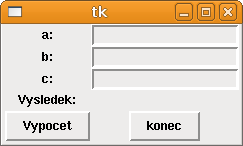
\includegraphics{img/tk2.png}}
  \end{center}
  \caption{Aplikace pro výpočet koeficientů kvadratické rovnice.}
  \label{fig:tk2}
\end{figure}

\subsection{Závěrem o GUI}
Tvorba GUI s sebou přináší jeden problém a to kvality návrhu rozhraní. Pro to, aby uživatel pracoval s GUI bez problémů, je nutné dodržovat zásady pro dobrý návrh aplikace. Toto je samozřejmě nad rámec toho to textu.

Knihovna Tk je samozřejmě mnohem obsáhlejší než bylo uvedeno výše. Můžete s ní jednoduše vytvářet i rozsáhlé aplikace, poněvadž počet komponent je široký. Vždyť dokumentace ke knihovně přesahuje 350 stran textu.



